\setchapterimage[6cm]{chapter/anime/Kiki.png}

\chapter{Anime: a mysterious and stunning world of Japanese animation\protect\footnotemark}

\labch{anime}

\footnotetext{\href{https://en.wikipedia.org/wiki/Krita\#Mascot}{Kiki}, an anime-styled \href{https://en.wikipedia.org/wiki/Mascot}{mascot} of Krita, free graphical editor. 
DeviantArt / \href{https://www.deviantart.com/tysontan/art/The-Magic-Stylus-570566846}{Tyson Tan} (CC-BY-SA 3.0)}

\marginnote[0.0cm]{Seiyu are the Japanese voice actors. Usually seiyu give voice to the characters of anime, video games, movies, work on the radio and TV. They act as storytellers on radio shows. Moreover, the seiyu's voices are used in advertisements, voice announcements, book audios and for re-sounding. Men and women, adults and children can work as seiyu.}

This chapter is dedicated to \wdqName{anime}{1107} Wikidata object analysis. Using SPARQL queries executed on Wikidata objects of anime type, several tasks were accomplished. The list that contains names of seiyu and number of their roles is shown, the histogram of seiyu that acted in one or more anime is presented, the graph that connects seiyu and anime voiced by them is constructed, the seiyu's activity age is estimated.

\section{Anime objects}

\begin{marginfigure}[0.0cm]
{
	\setlength{\fboxsep}{0pt}%
	\setlength{\fboxrule}{1pt}%
	\fcolorbox{gray}{gray}{
\includegraphics{chapter/anime/seyu.jpg}}
}
\caption
[Seiyu Kenji Akabane, 2021.]
{
Seiyu Kenji Akabane voiced the role of Sasuke Sarutobi in Ikemen Sengoku videogame, 2018.\newline
Wikimedia Commons / numan (CC BY-SA 3.0)
}
\label{fig:seiyu}
\end{marginfigure}

Anime is the Japanese animation. Anime has its unique visual style, but there are other features that are not that obvious. For instance, anime has a significantly wider variety of genres in comparison to the American and European animation: from family comedies and movies for kids to dramatic stories, whereas in the Western cinema the stories of such genre are mostly shown in the movies.

Each anime has its own voice actors. Here and further we will call the Japanese voice actors seiyu. In the Japanese animation the terms \emph{seiyu} and \emph{voice actor} are synonyms. Usually the word \emph{title} means the certain anime. In general \emph{title} means the term which combines different kinds of products, from cinema to novel, that are based on the same literary work which has an exact name.

In order to work with the anime list from Wikidata we need to use the \wdqName{anime}{1107} object and the \wdProperty{31}{instance of} property. Let's get the list of all anime names, without anime subclasses (listing~\protect\ref{lst:anime}).

\begin{lstlisting}[ language=SPARQL, breaklines=true, numbers=none,
                    caption={List of anime without subclasses. The result contained \num{683} instances of anime in 2017, 
                        \num{216} instances of anime in 2021.
                        SPARQL query: \href{https://w.wiki/4ABq}{w.wiki/4ABq}
                        },
                    label=lst:anime,
                    texcl 
                    ]
# List of instances of anime
SELECT ?anime ?animeLabel WHERE {
    ?anime wdt:P31 wd:Q1107. # instance of anime
    SERVICE wikibase:label{bd:serviceParam
					     wikibase:language "en,ja"}
}
\end{lstlisting}%

There are much more anime objects in Wikidata, but they are the instances not of anime, but of its subclasses, for example, \wdqName{anime series}{63952888}. Let's execute the query~\protect\ref{lst:anime_genres} in order to obtain the list of anime genres and the number of anime that correspond to these genres.

\begin{widepar}
\begin{lstlisting}[ language=SPARQL, breaklines=true, numbers=none,
                    caption={List of genres (subclasses) of anime. The result contained \num{11} genres of anime in 2021.
                        SPARQL query: \href{https://w.wiki/4ABt}{w.wiki/4ABt}
                        },
                    label=lst:anime_genres,
                    texcl 
                    ]
# Select anime and its subclasses with number of titles corresponding to these subclasses
SELECT ?subAnime ?subAnimeLabel (COUNT(?subAnimeInstance) AS ?count) WHERE {
  ?subAnime wdt:P279* wd:Q1107.
  ?subAnimeInstance wdt:P31 ?subAnime
   SERVICE wikibase:label {bd:serviceParam wikibase:language "en,ja"}
}
GROUP BY ?subAnime ?subAnimeLabel
ORDER BY DESC(?count)
\end{lstlisting}%
\end{widepar}

This classification of anime by genres is not perfect because there is a significant skewness to the anime television series: among \num{4875} titles, \num{2984} are the instances of anime series genre (\num{62,7}\%). Also, some subclasses correspond not to genres, but to the particular anime (i.e., \href{https://w.wiki/3iKe}{Evangelion}).

Let's get the list of all anime names including the titles that are the instances of anime subclasses, with script~\ref{lst:all_anime_list}.

\begin{lstlisting}[ language=SPARQL, breaklines=true, numbers=none,
                    caption={List of anime with the titles that are instances of anime subclasses.
                        The result contained \num{4875} anime names in 2021.
                        SPARQL query: \href{https://w.wiki/4ABv}{https://w.wiki/4ABv}
                        },
                    label=lst:all_anime_list,
                    texcl 
                    ]
# List of instances of anime and subclasses of anime
SELECT ?anime ?animeLabel
WHERE
{
    ?anime wdt:P31/wdt:P279* wd:Q1107.  # instance of anime
                                                              # with subclasses
    SERVICE wikibase:label{bd:serviceParam
					     wikibase:language "en,ja"}
}
\end{lstlisting}%

Anime that have the most complete information on Wikidata are \wdqName{Gurren Lagann}{4277}, \wdqName{Space Battleship Yamato}{4292}, \wdqName{Project A-ko}{4316}. There are also some anime with many missing properties like \wdqName{Doraemon}{711311}, \wdqName{The Animal Conference on the Environment}{97195557} and \wdqName{Assassins Pride}{96737300}.

% add Prowd link
According to ProWD service, among all the anime titles on Wikidata, \wdqName{Fullmetal Alchemist: The Sacred Star of Milos}{1004318}\sidenote{Fullmetal Alchemist: The Sacred Star of Milos is an anime movie which continues the Fullmetal Alchemist anime series. Its main characters are the alchemist brothers who use their magic to fight the criminals and forces of evil.} has the greatest number of properties (\num{24}).

\section{List of seiyu ordered by number of their roles in anime}

There are multiple characters in most of anime. Consequently, different seiyu give voice to different characters. Most of seiyu took part in multiple anime, but some of them managed to work on even several dozens of titles. Talented seiyu are sometimes offered to voice different charachers in one anime. \href{https://w.wiki/4UFa}{Hiroshi Kamiya} is one of the most popular modern seiyu. He worked on more than 180 anime and earned many rewards. \href{https://w.wiki/4UFh}{"Attack on Titan"} is one of the most famous anime with his participation where he dubbed captain Levi who is one of the main characters.

Let's create a sorted list of seiyu according to the number of anime voiced by them (listing~\protect\ref{lst:seiyu_titles_sorted}).

\begin{lstlisting}[ language=SPARQL, breaklines=true, numbers=none,
                    caption={Sorted list of seiyu according to the number of anime voiced by them.
                        \num{148} results in 2017, \num{2684} results in 2021.
                        SPARQL query: \href{https://w.wiki/4AC5}{https://w.wiki/4AC5}
                        },
                    label=lst:seiyu_titles_sorted,
                    texcl 
                    ]
# Ordered list of actors (seiyu) according to the number
# of anime where they took part in.
SELECT ?seiyu (SAMPLE(?label) AS ?seiyuLabel)
(COUNT(?anime) AS ?count) WHERE {
  # instance of anime/subclass
  ?anime wdt:P31/wdt:P279* wd:Q1107;
         wdt:P725 ?seiyu.  # instance of seiyu (voice actor)
  ?seiyu rdfs:label ?label	# subclass of label
  SERVICE wikibase:label{bd:serviceParam
					   wikibase:language "en,ja"}
}
GROUP BY ?seiyu		 # group by seiyu 
ORDER BY DESC(?count)	# order by number of voiced anime
\end{lstlisting}%

\section{Chart of number of seiyu who worked on one or more anime}

We can create a line chart of seiyu according to the number of their roles. The more anime the seiyu has voiced, the more to the right he is on the diagram. We can use the script~\protect\ref{lst:seiyu_titles_graph} to create the chart.

\begin{lstlisting}[ language=SPARQL, breaklines=true,
                    caption={Display the line chart with the seiyu number along X-axis and anime number along Y-axis.
                        \num{13} results in 2017, \num{58} results in 2021.
                        SPARQL query: \href{https://w.wiki/4UX8}{https://w.wiki/4UX8}
                        },
                    label=lst:seiyu_titles_graph,
                    texcl 
                    ]
# Graph of the number of voice actings of different seiyu
#defaultView:LineChart
SELECT ?seiyuRoles (COUNT(?seiyuRoles) AS ?quantity) WHERE {
  FILTER(?seiyuRoles < 71)
  {
     SELECT (COUNT(?seiyu) AS ?seiyuRoles) WHERE {
       ?anime wdt:P31/wdt:P279* wd:Q1107;
              wdt:P725 ?seiyu.
       SERVICE wikibase:label { bd:serviceParam wikibase:language "en,ja"}
     }
     GROUP BY ?anime
     ORDER BY DESC(?seiyuRoles)
  }
}
GROUP BY ?seiyuRoles
ORDER BY DESC(?seiyuRoles)
}
\end{lstlisting}%

Fig.~\ref{fig:Seiyu_num_chart_2021_en} shows that the higher the number of voiced anime is, the less seiyu reach such number of roles. The line \num{4} of script~\protect\ref{lst:seiyu_titles_graph} sets the limit of \num{71} anime as there are only few seiyu that worked on bigger number of anime, and the graph expansion to the right wouldn't be informative.

As the chart~\ref{fig:Seiyu_num_chart_2021_en} shows, most of the seiyu voiced only one anime during their life. There are \num{254} seiyu with one role in the chart. However, seiyu is a profession which becomes the life business for people. The fact that a person voiced only one role in his life according to Wikidata seems to be caused by the incompleteness of Wikidata.

\begin{figure*}[h]

    \setlength{\fboxsep}{0pt}%
    \setlength{\fboxrule}{1pt}%
    \fcolorbox{gray}{gray}{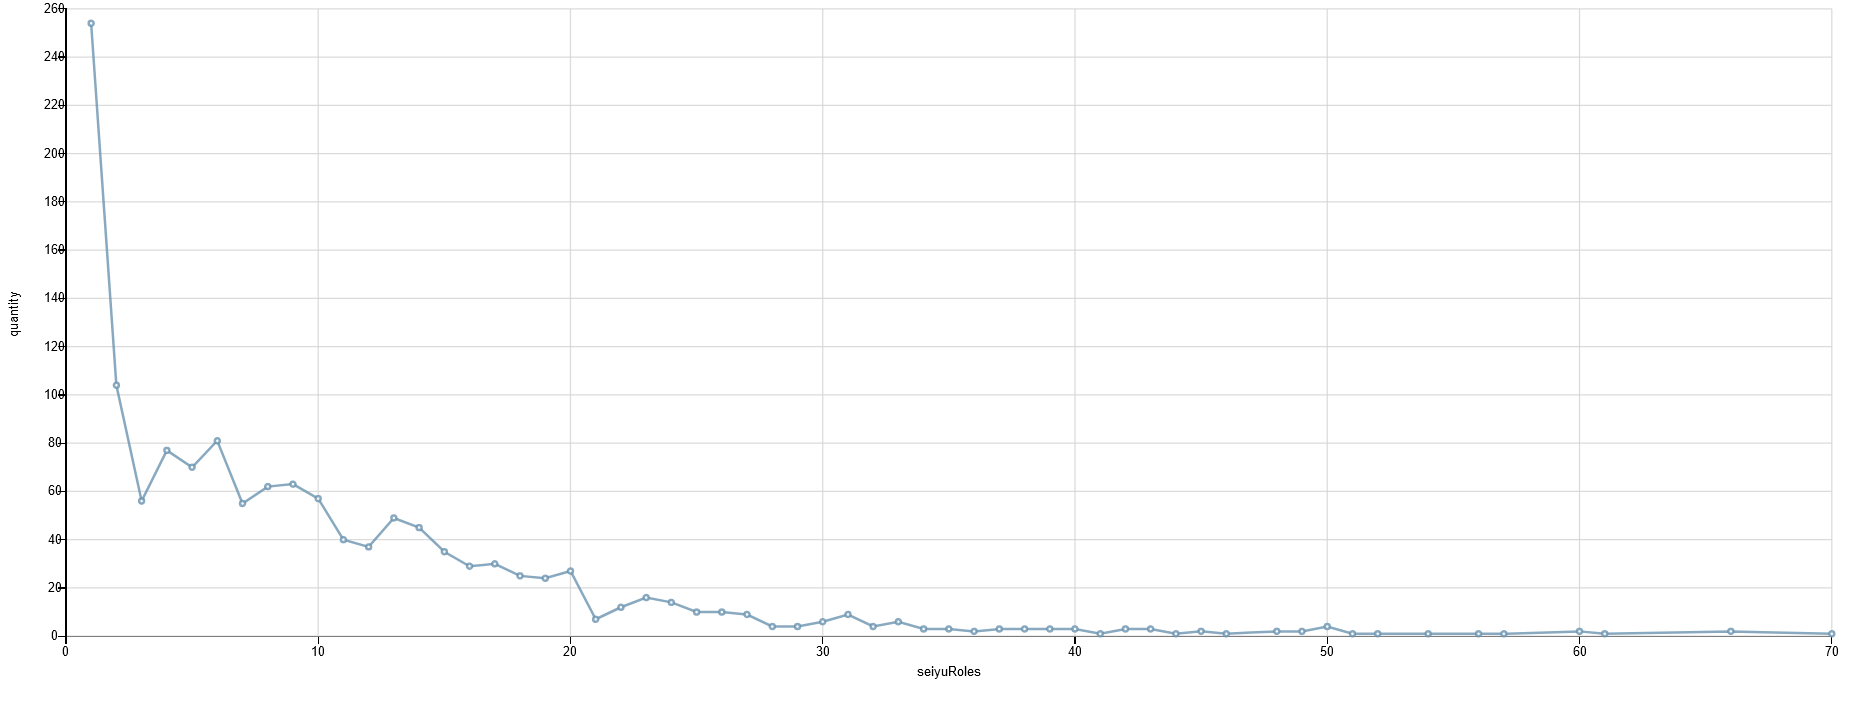
\includegraphics[width=\linewidth]{chapter/anime/Seiyu_chart_2021_en.png}}
	\caption[Chart of number of roles voiced by different seiyu, 2021.]{Chart of number of roles voiced by different seiyu, 2021. The chart is constructed using the output of script~\protect\ref{lst:seiyu_titles_graph}.}%
    \label{fig:Seiyu_num_chart_2021_en}%
\end{figure*} 